%%=============================================================================
%% Proof-of-concept van een CI/CD pipeline
%%=============================================================================

\chapter{\IfLanguageName{dutch}{Proof-of-concept van een CI/CD pipeline}{Setting up a CI/CD pipeline}}
\label{ch:proof-of-concept}
Uit vorig hoofdstuk is gebleken dat (SCHRAPPEN WAT NIET PAST): Jenkins \& Travis \& Bamboo de tools zijn die aan het meeste must-haves, should-haves en nice-to-haves voldoen. In dit hoofdstuk worden deze tools extra onder de loep genomen door ze op te stellen in een realistische omgeving zoals in hoofdstuk/ref{ch:voorbeeldapplicatie} besproken is. Door de tools te vergelijken in zo'n omgeving krijgen we een meer realistisch beeld welke build-scheduler het beste zal functioneren in deze omgeving. Op het einde van dit hoofdstuk zal er een conclusie worden gemaakt welke build-scheduler Amista moet kiezen en waarom. Maar beginnen doen we met enkele tips te geven van SAP hoe een CI/CD pipeline opgestart moet worden.

\section{Continuous Delivery principles}
\label{sec:continuous-delivery-principles}
Volgens \textcite{Riti2018} is het uitermate belangrijk om volgende stappen te volbrengen om tot een goede Continuous Delivery omgeving te komen.
\begin{itemize}
    \item Er moeten goede branching strategieën bepaald worden om het team goed te laten samenwerken
    \item Een belangrijk onderdeel van Continuous Integration is natuurlijk testen, deze zijn in Continuous Delivery niet te vergeten
    \item Een stap verder is het automatisch uitvoeren van deze testen
    \item Na het slagen van de testen en het automatisch builden van de software moet de build klaar gemaakt worden voor release
\end{itemize}

\section{CI/CD pipeline op SAP Cloud Platform}
\label{sec:ci-cd-op-sap-cloud-platform}
SAP Cloud Platform biedt de mogelijkheid om verschillende omgevingen op te stellen waarin je kan werken als developer. Het vergt enige vereisten om te voldoen aan de regels van Continuous Integration ~\autocite{Kramer2018}:
\begin{itemize}
    \item Hou alles goed bij via een version control systeem
    \item Automatiseer de build
    \item Zorg ervoor dat tijdens de build er Unit testen lopen
    \item Het team moet op regelmatige basis commits uitvoeren
    \item Elke verandering moet gebuild worden
    \item Als er errors tevoorschijn komen tijdens de build, moeten die opgelost worden
    \item De build moet uitgetest worden op een kopie van de productieomgeving
    \item Automatiseer de deployment
\end{itemize}
Eens deze regels zijn toegepast, kunnen we spreken van een CI implementatie.
Vaak wordt CI in combinatie gebracht met Continuous Delivery. Om dit in een vloeiende lijn te laten lopen, spreekt men van een CI/CD pipeline.

\section{CI/CD pipeline volgens SAP}
\label{sec:ci-cd-pipeling-volgens-sap}
SAP is een Duitse onderneming dat softwareoplossingen aanbiedt voor grote ondernemingen en heeft zicht gespecialiseerd in het maken van ERP pakketten. Dat is software dat alle processen van het bedrijf opneemt ~\autocite{SAPERP2019}.
Een programmeur schrijft nieuwe code voor een verandering die de klant wil uitvoeren. Idealiter zou dit - voor het mergen naar de masterapplication - eens door een voter build moeten gaan, waar automatische tests aanwezig zijn die kijken of de code geen problemen zou geven als je die zou mergen met de master. Een laatste stap voor de code naar de master gemerged wordt, is het toepassen van code reviews door collega developers (het 4-ogen principe).
Na het samenvoegen wordt automatisch de CI-build geactiveerd. De code gaat door de automatische tests. Eens de testen slagen worden de wijzigingen geïntegreerd op de master. 

Dan komt de Continuous Delivery fase, waarbij de code nog eens door een testsysteem gaat. Deze fase gebeurt volledig automatisch, maar er kunnen ook manueel testen uitgevoerd worden. Eens de code door deze fase raakt, is ze klaar om te deployen. 
Bij Continuous Deployment worden de wijzigingen dus automatisch naar buiten gebracht ~\autocite{Kramer2018}.

\section{Automated Tests voor CI}
\label{sec:automated-test-voor-ci}
Om te zorgen dat de automated tests aan de noden van Continuous Integration voldoen, moet er rekening gehouden worden met enkele criteria: snelheid, betrouwbaarheid, hoeveelheid en onderhoud.
Bij Continuous Integration draait alles rond feedback, hierbij speelt snelheid een niet te onderschatten rol. Wanneer het runnen van de automated tests enige tijd vergt, zal de developer pas laat feedback terug krijgen waar de pipeline gefaald is. Daarom is het belangrijk rekening te houden met de test piramide bij het ontwerpen van de test omgeving. Er moet telkens een goede afweging gemaakt worden in welke categorie elke test gestoken kan worden.
~\autocite{Jones2019}.

Betrouwbaarheid wordt tegenwoordig als 'normaal' beschouwd, maar dit is niet zo vanzelfsprekend. Het kan gebeuren dat de automated tests niet zo betrouwbaar zijn waardoor de developers met valse informatie moeten werken. Dit is niet bevorderlijk voor de verdere productie en het vertrouwen in een Continuous Integration en Continuous Delivery pipeline. Er zijn wel enkele tips om de automated tests betrouwbaar te maken door de UI elements een degelijke identifier geven. Zo hoeven de testen niet de onbetrouwbare css selectors te gebruiken om aan de elementen te kunnen. 

De test data onderhouden is ook een belangrijke tip. Dit kan door één bron van informatie te voorzien voor test data, vooral in het bijzonder wanneer testen - die dezelfde data aanpassen en controleren - tegelijk runnen. Rekening houden met de asynchrone acties bij Service en UI tests uit de Test Pyramid (Figuur \ref{img-test-pyramid}) door bepaalde situaties te vermijden. We hebben het over situaties waarbij de applicatie zich in de verkeerde staat bevindt, zodat de asynchrone test foute resultaten teruggeeft.

De hoeveelheid aan tests moet beperkt blijven om zo de snelheid van de execution times, de hoge waarde van tests en het onderhoudsgemak te bewaren.
Als men automated tests schrijft voor een CI/CD pipeline, moet men zaken testen die de integratie en het deployen van de applicatie kunnen verstoren.
Ook kritieke functionaliteiten, nieuwe informatie, zaken die de voorbije builds fout liepen moeten getest worden. 
De testen groeperen per functionaliteit is een goede tip, zo moet er niet telkens elke functionaliteit opnieuw getest worden. Maar kan de build scheduler beslissen welke groep test moet runnen bij de nieuwe code. 
Angie Jones \textcite{Jones2019} geeft ook nog als tip mee om af en toe wat onnodige testen te verwijderen.

Voor het onderhoud van de testen moet je rekening houden met de staat van je applicatie. Deze verandert doorheen de tijd en je testen moeten deze verandering ook doorstaan.

    \paragraph{Testing in SAPUI5}
    De developers van SAP hebben ook eigen test-frameworks ontwikkeld. Voor Unit testen zijn er de QUnit tests en voor de integratie testen hebben ze OPA, One-Page Acceptance Test, ontwikkeld.
    %TODO: https://blogs.sap.com/2018/10/03/testing-your-sapui5-application-with-opa5/
    %TODO: Automatic testing with OPA on Jenkins and Travis: https://stackoverflow.com/questions/24934012/automated-ui-tests-for-sap-ui5 (onderste post)
    %TODO: https://github.com/SAP/karma-ui5/issues/1

\section{Short List}
\label{sec:short-list}
Uit het hoofdstuk\ref{ch:methodologie} hebben we in grote lijnen de vergelijking gemaakt tussen verschillende build schedulers. Hier gaan we een gedetailleerde vergelijking te maken door de build schedulers uit te testen aan de hand van de voorbeeldapplicatie die uitgewerkt is in hoofdstuk\ref{ch:methodologie}.
We hebben Jenkins en %TODO: volgende tool gekozen om uit te zetten en te vergelijken met elkaar.
In het vorige hoofdstuk hebben we de Ubuntu server helemaal klaar gezet voor het gebruik met een build scheduler. De opzet van Jenkins en %TODO: andere buikd scheduler
wordt hier beschreven.

    \paragraph{Jenkins}
    Omdat Jenkins op Java draait is het nodig om Java 8 te installeren. Dit is dan ook de eerste stap in het proces. 
    De eerste stap is inloggen in de server door ssh root@188.166.61.128 in te typen. Daarna moet je het commando sudo apt install openjdk-8-jdk intypen om JAVA 8 te installeren. De server vraagt bevestiging om te downloaden en te installeren, er moet enkel maar y worden getypt en op return gedrukt worden om te bevestigen. Dit kan u zien in figuren \ref{InstallatieJenkins1} en \ref{InstallatieJenkins2}.
    Nu kunnen we overgaan tot de installatie van Jenkins op de server. We maken gebruik van de packages die Jenkins onderhoud om de software te installeren op Ubuntu zoals te zien is in figuur \ref{InstallatieJenkins3}.
    Eens dit gebeurd is moeten we de Debian package repository toevoegen aan de server's sources.list.
    De apt - een command-line tool binnen Ubuntu om software te installeren - moet eerst geupdate worden, nadien kan Jenkins effectief geïnstalleerd worden. Deze stappen kan u volgen in figuren \ref{InstallatieJenkins4} en \ref{InstallatieJenkins5}.
    
    \begin{figure}	
        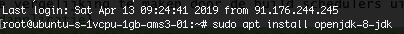
\includegraphics{InstallatieJenkins1}
        \caption{Installatie Jenkins, stap 1} \label{InstallatieJenkins1}
    \end{figure}
    
    \begin{figure}	
        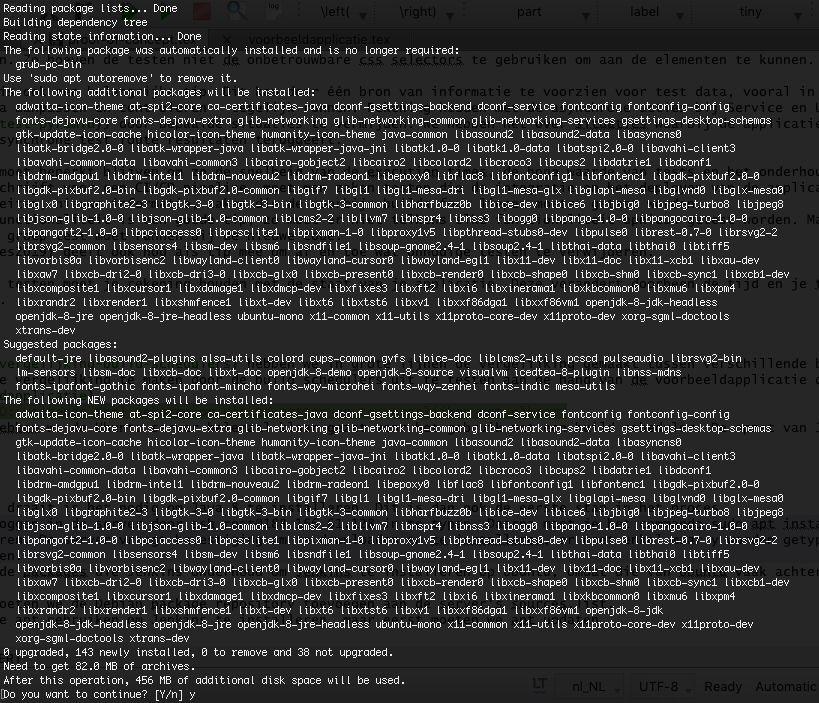
\includegraphics{InstallatieJenkins2}
        \caption{Installatie Jenkins, stap 2} \label{InstallatieJenkins2}
    \end{figure}
    
    \begin{figure}	
        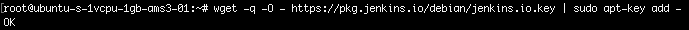
\includegraphics{InstallatieJenkins3}
        \caption{Installatie Jenkins, stap 3} \label{InstallatieJenkins3}
    \end{figure}
    
    \begin{figure}	
        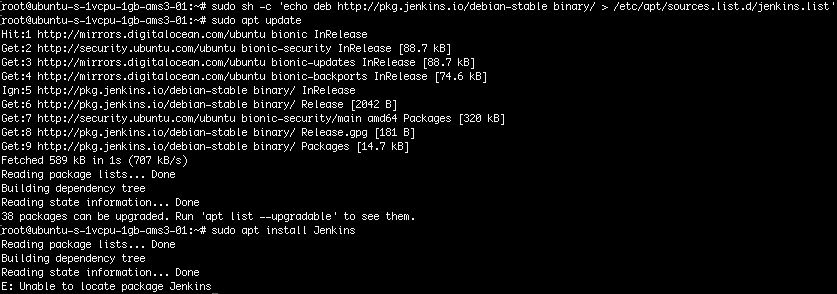
\includegraphics{InstallatieJenkins4}
        \caption{Installatie Jenkins, stap 4} \label{InstallatieJenkins4}
    \end{figure}
    
    \begin{figure}	
        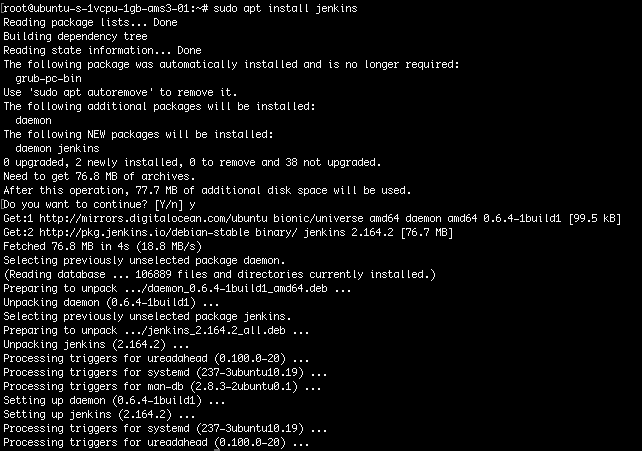
\includegraphics{InstallatieJenkins5}
        \caption{Installatie Jenkins, stap 5} \label{InstallatieJenkins5}
    \end{figure}

    
    Na de installatie kunnen we Jenkins starten op de server door het commando 'sudo systemctl start jenkins' in te typen. Omdat dit commando geen uitvoer geeft moeten we het commando 'sudo systemctl status jenkins' intypen. Als je active ziet verschijnen wil dit zeggen dan Jenkins runt op de Ubuntu server. Deze stappen kan je volgen in figuur \ref{Jenkins1}.
    Eens Jenkins gestart is moeten we die kunnen aanspreken vanuit een browser, daarom moeten we de regels van de firewall wat aanpassen. Standaard draait Jenkins op poort 8080. Deze moet geopend worden op de server door het commando 'sudo ufw allow 8080' in te voeren zoals in figuur \ref{Jenkins2} te zien is.
    
    Nu moet Jenkins geconfigureerd worden, dit moet vanuit elke browser gebeuren.
    Er moet naar http://188.166.61.128:8080 gesurft worden om de configuratie te voltooien, zoals aangegeven in figuur \ref{Jenkins3}. De cijfers voor de :8080 staan voor het ip-adres van de Ubuntu server, de :8080 is de poort waar je naartoe wil gaan. Hier draait - zoals in de vorige stappen geconfigureerd - Jenkins op.
    Het paswoord dat gevraagd wordt is terug te vinden in de 'initialAdminPassword' file dat zich in de map '/var/lib/jenkins/secrets/' bevindt op de server. Het is voldoende om op de server volgend commando in te voeren: 'sudo cat /var/lib/jenkins/secrets/initialAdminPassword'. Het paswoord dat als uitvoer komt moet gekopieerd worden en geplakt worden in het invoerveld in de web browser zoals in figuur \ref{Jenkins4} te zien is.
    De volgende stap is het installeren van de voorgestelde plugins. Er wordt gevraagd om een eerste user te configureren, maar voor deze doeleinden is het voldoende om als admin en met het initiële paswoord verder te gaan, er mag dus op 'Continue as admin' gedrukt worden. Nu moet er instantie gemaakt worden door te controleren of de url die ingevuld is klopt met de url die enkele stappen geleden ingegeven is om de webpagina te openen. Wanneer deze klopt kan er op 'Save and Finish' en nadien op 'Start using Jenkins' geklikt worden. Het dashboard van Jenkins wordt geopend. Bovenstaande stappen kan u allemaal volgen in de figuren \ref{Jenkins5}, \ref{Jenkins6}, \ref{Jenkins7}, \ref{Jenkins8}, \ref{Jenkins9} en \ref{Jenkins10}.
    
    \begin{figure}	
        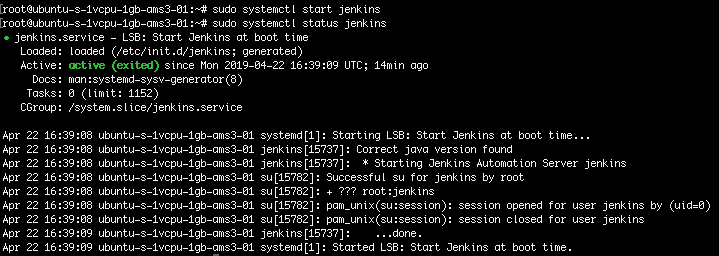
\includegraphics{Jenkins1}
        \caption{Opzetten Jenkins, stap 1} \label{Jenkins1}
    \end{figure}
    
    \begin{figure}	
        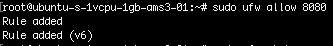
\includegraphics{Jenkins2}
        \caption{Opzetten Jenkins, stap 2} \label{Jenkins2}
    \end{figure}
    
    \begin{figure}	
        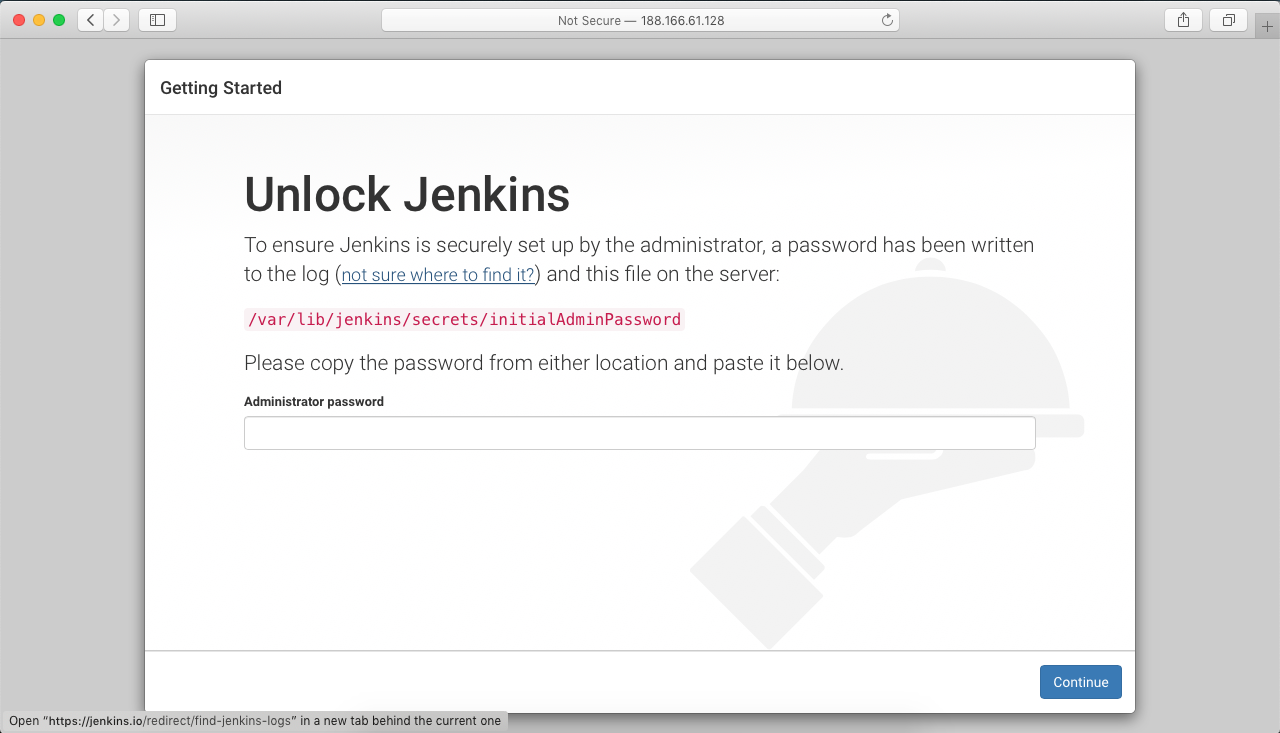
\includegraphics{Jenkins3}
        \caption{Opzetten Jenkins, stap 3} \label{Jenkins3}
    \end{figure}
    
    \begin{figure}	
        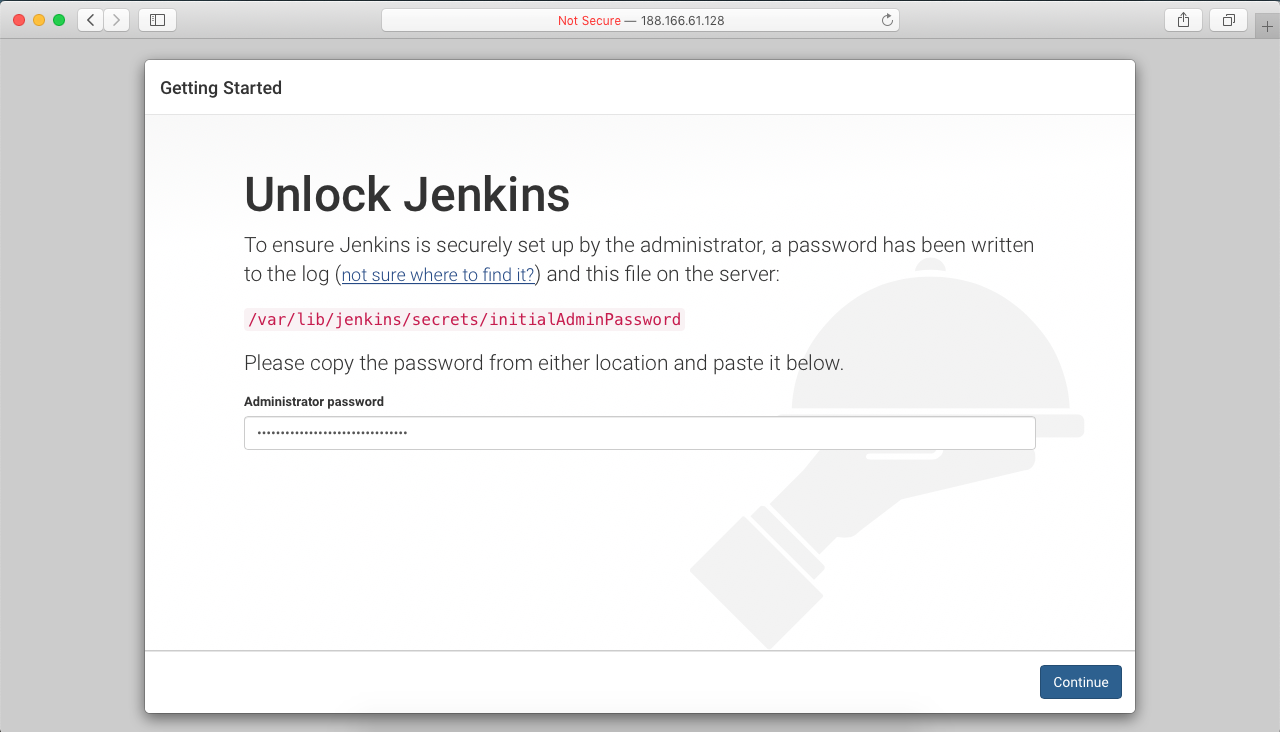
\includegraphics{Jenkins4}
        \caption{Opzetten Jenkins, stap 4} \label{Jenkins4}
    \end{figure}
    
    \begin{figure}	
        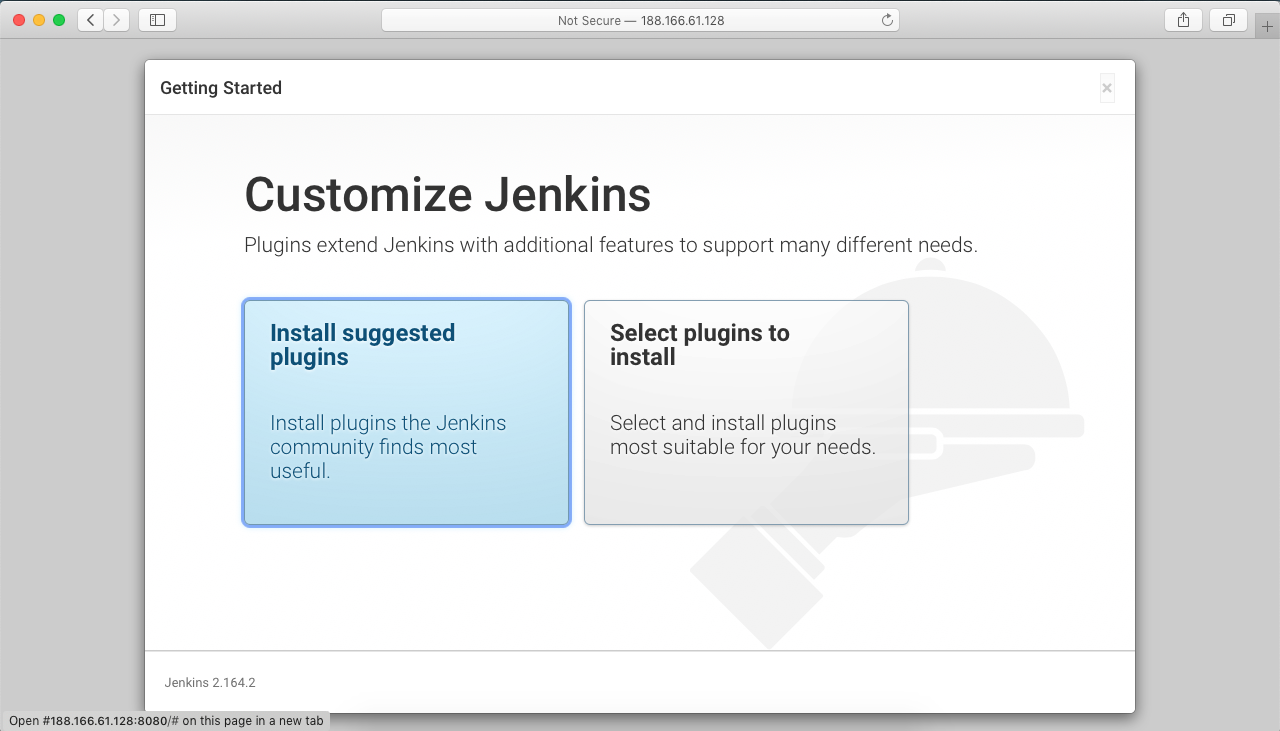
\includegraphics{Jenkins5}
        \caption{Opzetten Jenkins, stap 5} \label{Jenkins5}
    \end{figure}
    
    \begin{figure}	
        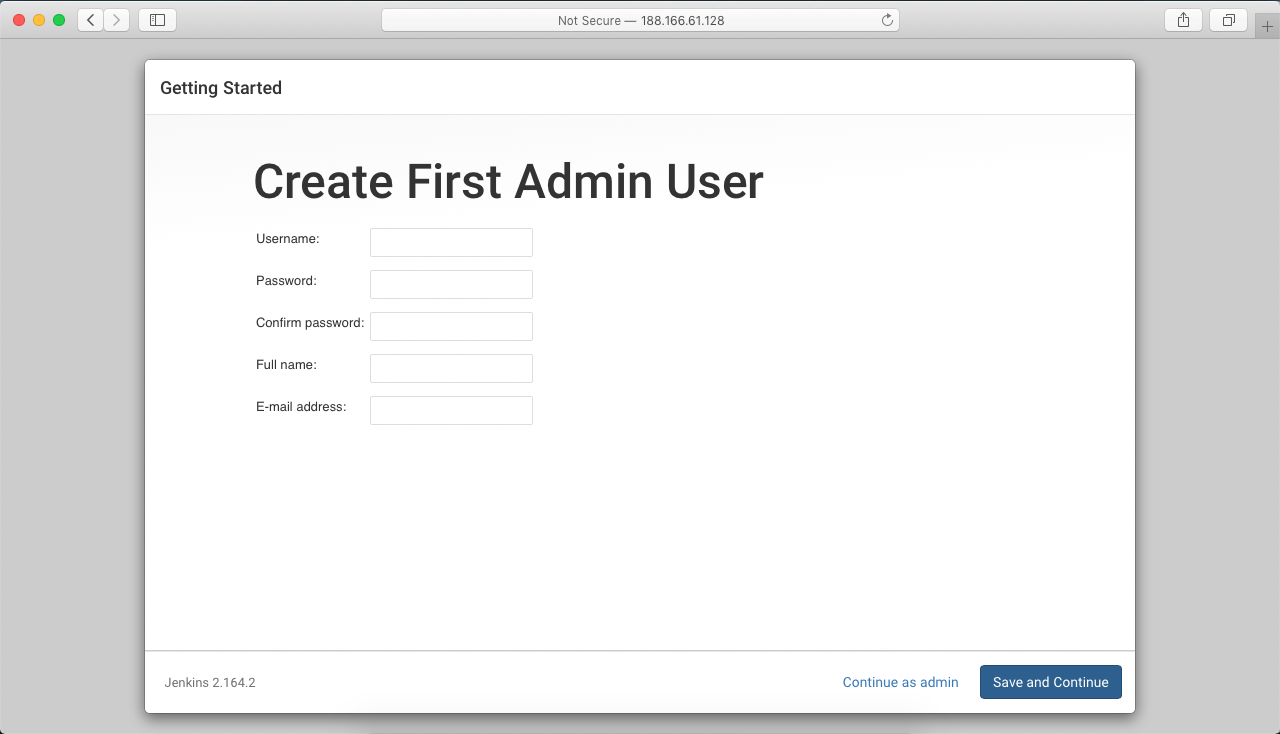
\includegraphics{Jenkins6}
        \caption{Opzetten Jenkins, stap 6} \label{Jenkins6}
    \end{figure}

    \begin{figure}	
        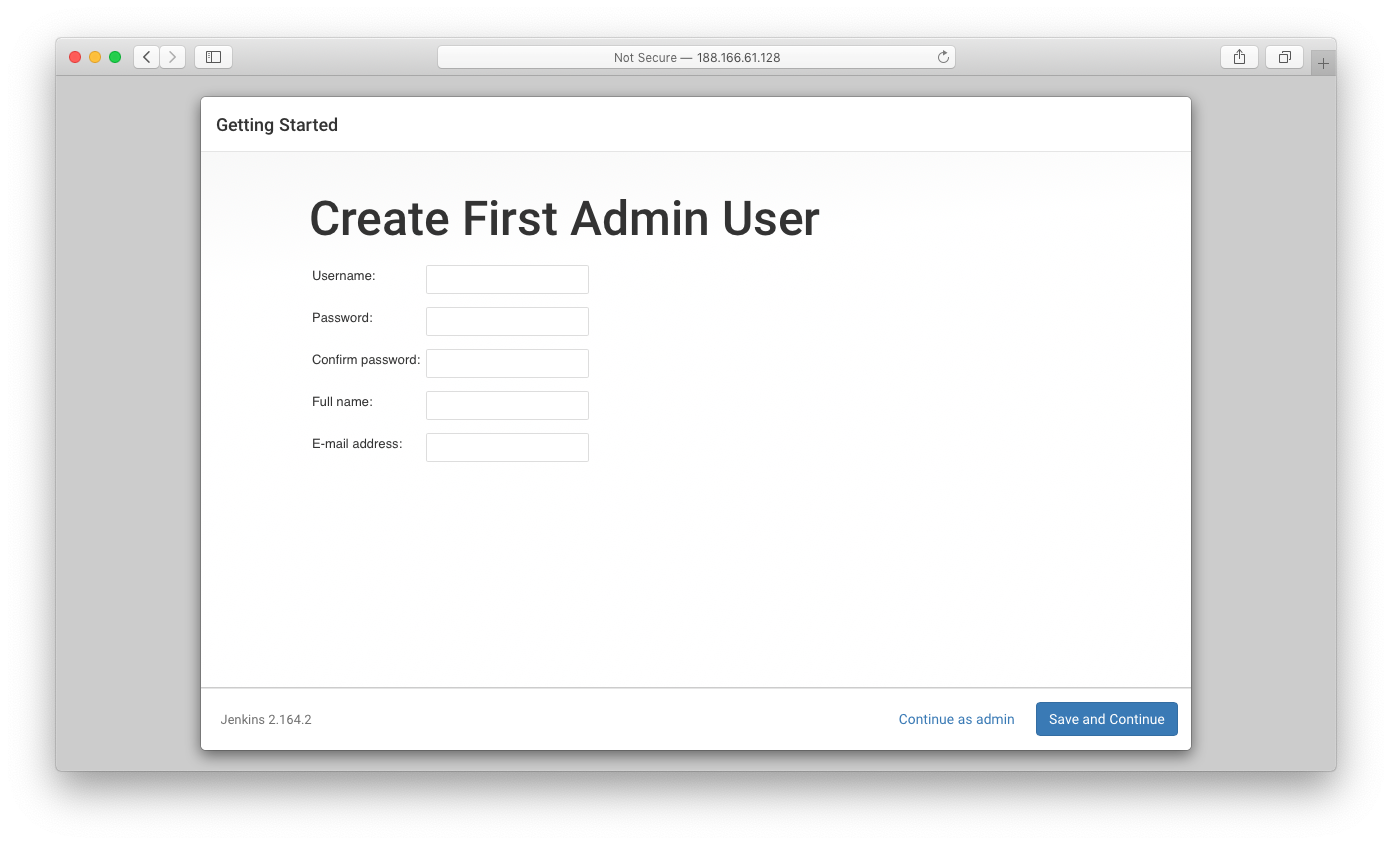
\includegraphics{Jenkins7}
        \caption{Opzetten Jenkins, stap 7} \label{Jenkins7}
    \end{figure}
    
    \begin{figure}	
        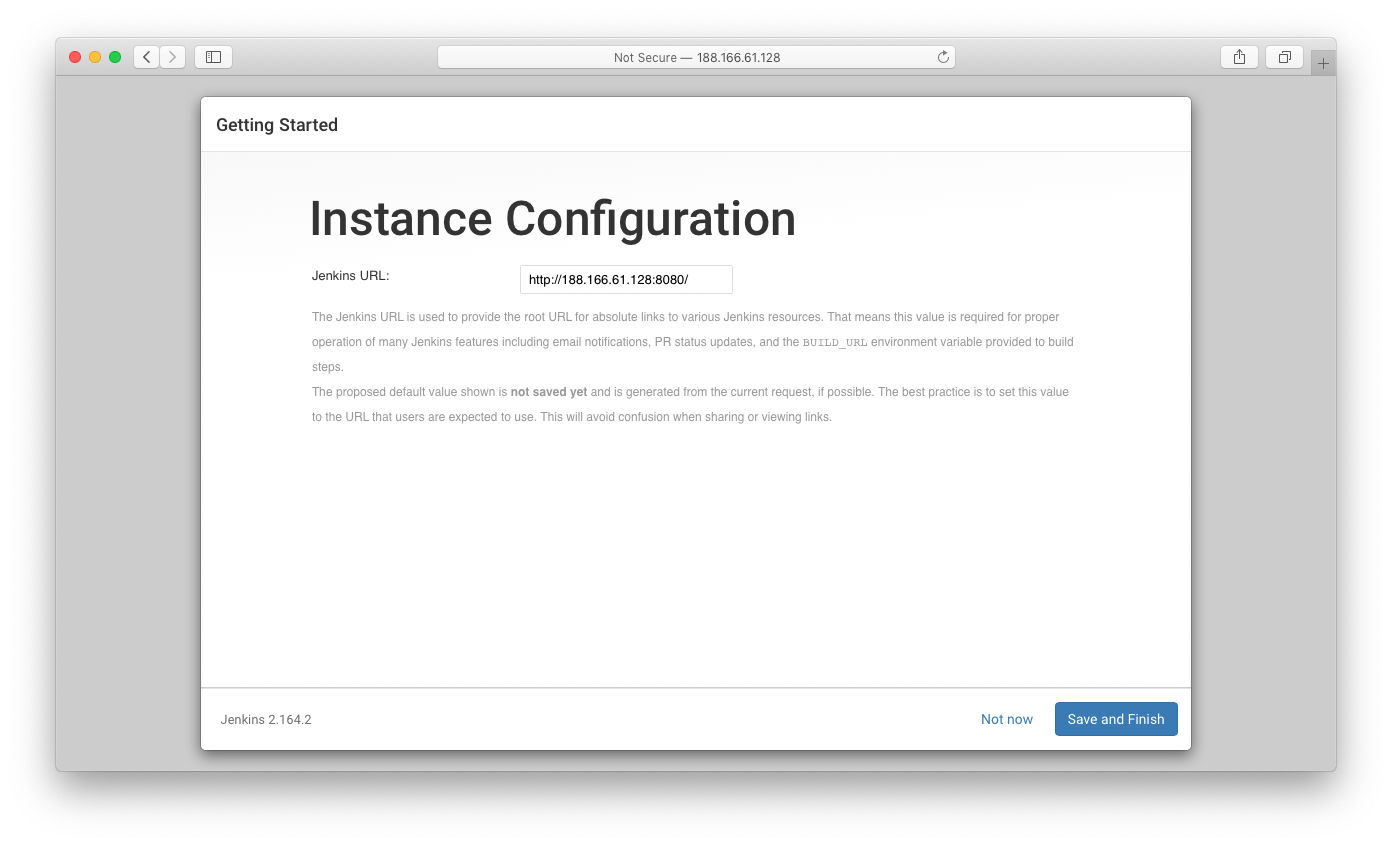
\includegraphics{Jenkins8}
        \caption{Opzetten Jenkins, stap 8} \label{Jenkins8}
    \end{figure}
    
    \begin{figure}	
        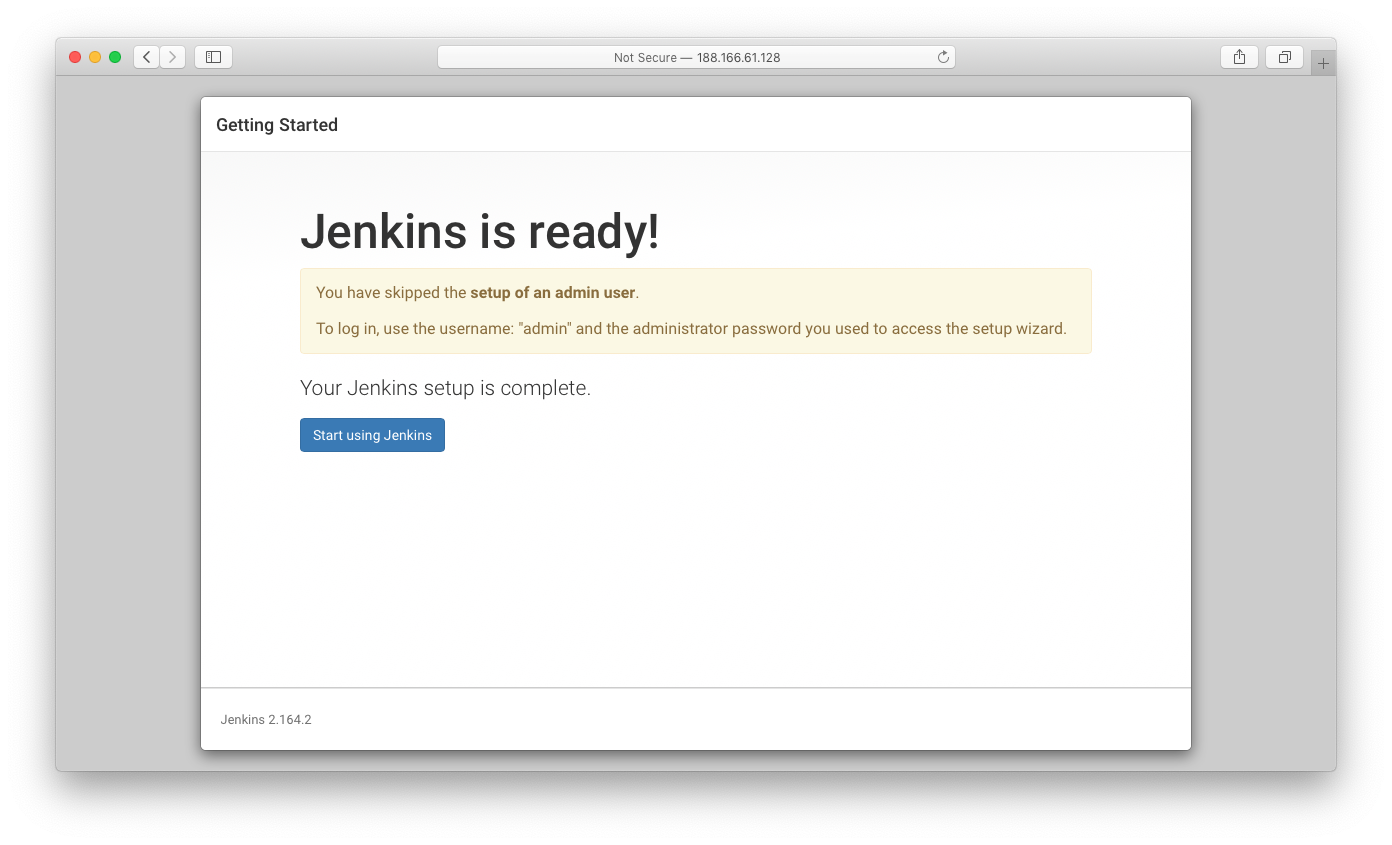
\includegraphics{Jenkins9}
        \caption{Opzetten Jenkins, stap 9} \label{Jenkins9}
    \end{figure}
    
    \begin{figure}	
        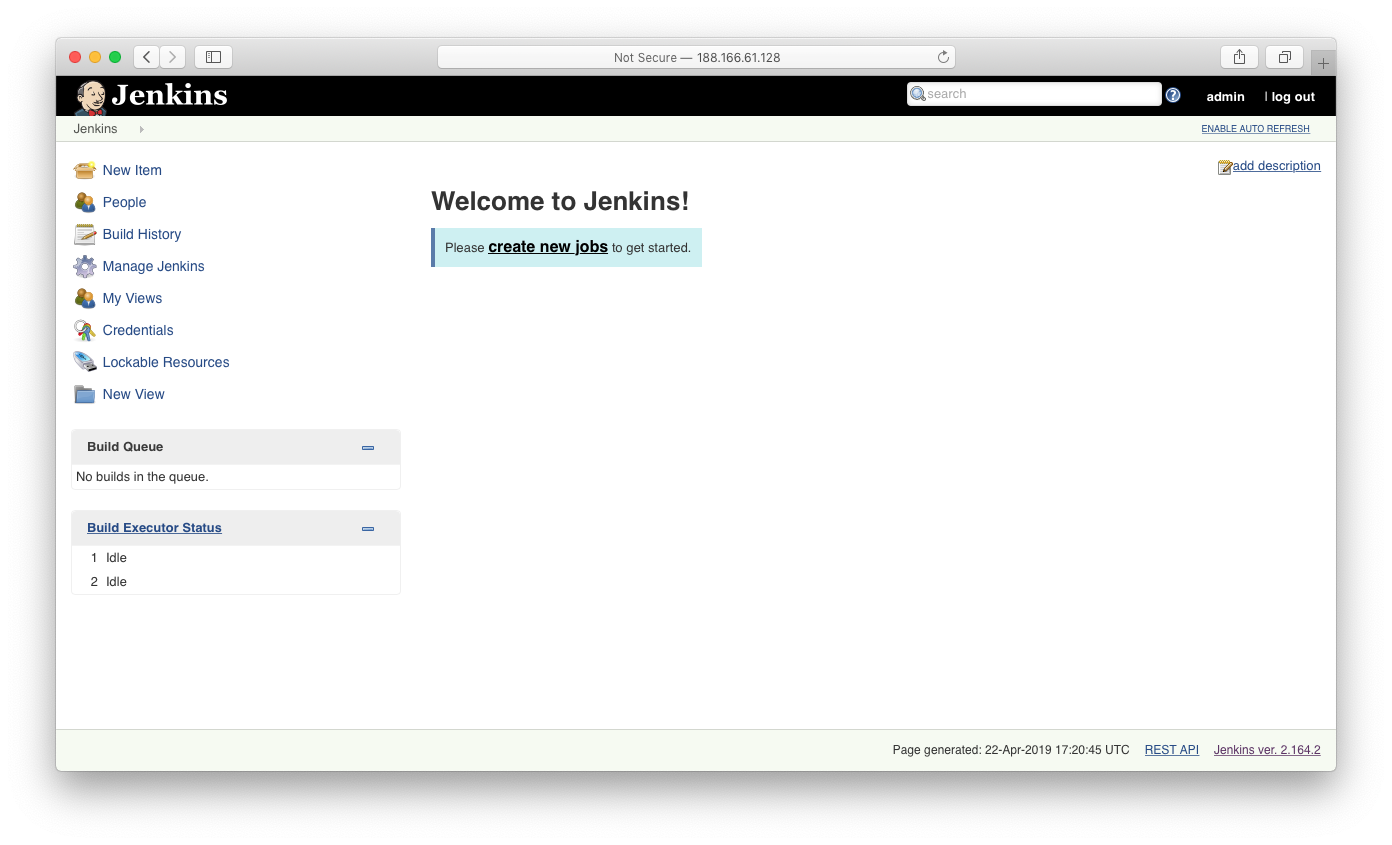
\includegraphics{Jenkins10}
        \caption{Opzetten Jenkins, stap 10} \label{Jenkins10}
    \end{figure}
    
    %TODO: https://sap.github.io/jenkins-library/scenarios/ui5-sap-cp/Readme/!!!!!!!!!
    %TODO: https://blogs.sap.com/2017/11/21/continuous-delivery-with-jenkins-pipelines/
    %TODO: http://www.sapspot.com/ci-cd-for-sapui5-on-scp-neo-with-gitlab/
    %TODO: OPA test via Selenium: https://www.agiletrailblazers.com/blog/modernized-technology/automated-testing-with-selenium-grid-and-jenkins-in-3-steps
    
    
\section{Conclusie}
\label{sec:conclusie}
